% 多维球体的体积

\pentry{定积分\upref{DefInt},$\Gamma$ 函数\upref{Gamma}}
\subsection{结论}
\begin{equation}
V_n = \leftgroup{
& \frac{R^n}{(n/2)!} \pi^{(n - 1)/2} && (n = 2n-1)\\
&\frac{R^n}{(n/2)!} \pi^{n/2} && (n = 2n)
} = \frac{\pi^{n/2} R^n}{\Gamma (1 + n/2)}
\end{equation}
 
\subsection{说明}
若定义 $n$ 维球体的表面满足方程 $\sum_{i=1}^n x_i^2 = R_n^2$, 其中 $x_i$ 为 $n$ 维直角坐标系中第 $i$ 个坐标.所有满足 $\sum_{i=1}^n x_i^2 \les R_n^2$ 的坐标点都定义为球内的点,且定义 $n$ 维直角坐标系中的体积为 $V_n = \int \dd{x_1}\dd{x_2}\dots\dd{x_n}$, 积分是对所有球内的点积分.

如果这些定义看起来很抽象,不妨代入到三维空间中考虑.三维直角坐标系中, $x_1, x_2, x_3$ 分别是 $x,y,z$,  $R_3$ 是球的半径,球表面上任意一点都满足 $x^2 + y^2 + z^2 = R_3^2$, 且球的体积分为 $\int \dd{x}\dd{y}\dd{z}$ 是对球内部的所有点积分. 另外,若把上述定义代入到 1 维和 2 维, 不难发现所谓的“1 维球”和“2 维球”分别是半径为 $R_1$ 的线段和半径为 $R_2$ 的圆.

\subsection{推导}
由于正常人的空间想象力最高是 3 维,我们先由 3 维以内的球体总结出体积的递推公式,这样即使我们无法想象高维球的形状,也可以计算其体积.下面在推导前 3 个维度时,请把所有 $x_1, x_2, x_3$ 想象成 $xyz$. 
\begin{figure}[ht]
\centering
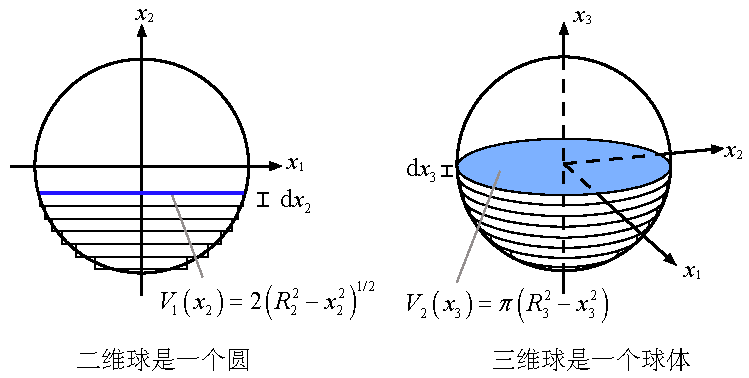
\includegraphics[width=12cm]{./figures/NSphV1.pdf}
\caption{二维和三维球的体积}
\end{figure}
\subsection{1 维球}
这是一条线段,满足 $x_1^2 \les R_1^2$, “体积”就是线段长度
\begin{equation}\label{NSphV_eq1}
V_1 = \int \dd{x_1} = 2 R_1
\end{equation}
\subsection{ 2 维球}
这是一个圆,满足 $x_1^2 + x_2^2 \les R_2^2$, 在计算体积 $V_2 = \int \dd{x_1}\dd{x_2}$ 时,可以先对 $x_1$ 积分再对 $x_2$ 积分
\begin{equation}\label{NSphV_eq2}
V_2 = \int \qty(\int \dd{x_1}) \dd{x_2}  = \int V_1(x_2) \dd{x_2}
\end{equation}
在几何上,这就是说把圆从沿 $x_1$ 轴切成许多一维球(线段),由 $x_1^2 \les R_2^2 - x_2^2$, 一维球的半径为 $R_1(x_2) = (R_2^2 - x_2^2)^{1/2}$. 代入\autoref{NSphV_eq1}, 得 $x_2$ 处切出的一维球的体积(线段的长度)为
\begin{equation}\label{NSphV_eq3}
V_1 (x_2) = \int \dd{x_1} = 2R_1 = 2(R_2^2 - x_2^2)^{1/2}
\end{equation}
再代入\autoref{NSphV_eq2}, 得二维球的体积为(注意 $ -R_2 < x_2 < R_2$ )
\begin{equation}\label{NSphV_eq4}
V_2 = \int V_1 \dd{x_2} = \int 2 (R_2^2 - x_2^2)^{1/2} \dd{x_2}  = \pi R_2^2
\end{equation}
\subsection{ 3 维球}
这是一个球体,满足 $x_1^2 + x_2^2 + x_3^2 \les R_3^2$, 计算体积 $V_3 = \int \dd{x_1}\dd{x_2} \dd{x_3}$ 时,可以先对 $x_1 x_2$ 积分
\begin{equation}\label{NSphV_eq5}
V_3 = \int \qty(\int \dd{x_1} \dd{x_2}) \dd{x_3} = \int V_2(x_3) \dd{x_3}
\end{equation}
在几何意义上,这是说把球沿 $x_1 x_2$ 平面切成许多二维球(圆),然后把球的体积(面积)沿 $x_3$ 轴积分.由 $x_1^2 + x_2^2 \les R_3^2 - x_3^2$, 得 $x_3$ 处二维球半径为 $R_2 = (R_3^2 - x_3^2)^{1/2}$. 由\autoref{NSphV_eq4} 得体积为
\begin{equation}\label{NSphV_eq6}
V_2 (x_3) = \pi R_2^2 = \pi (R_3^2 - x_3^2)
\end{equation}
代入\autoref{NSphV_eq5} 得三维球体积(注意 $-R_2 < x_2 < R_2$)
\begin{equation}\label{NSphV_eq7}
V_3 = \int V_2(x_3) \dd{x_3} = \int \pi (R_3^2 - x_3^2)\dd{x_3}  = \frac43 \pi R^3
\end{equation}
\subsection{ $n$ 维球}
由以上两个推导,可以在代数上总结出递推的规律.把 $n$ 维球在 $n+1$ 维积分,得(可使用  Mathematica 软件计算积分,见 Mathematica 积分)%未完成:链接
\begin{gather}
V_4 = \int_{-R}^R \frac43 \pi (R_4^2 - x_4^2)^{3/2} \dd{x_4}  = \frac12 \pi^2 R^4\\
V_5 = \int_{-R}^R \frac12 \pi^2 (R_5^2 - x_5^2)^{4/2} \dd{x_5}  = \frac{8}{15} \pi^2 R^5\\
V_6 = \int_{-R}^R \frac{8}{15} \pi ^2 (R_6^2 - x_6^2)^{5/2} \dd{x_6} = \frac16 \pi^3 R^6\\
V_7 = \int_{-R}^R \frac16 \pi^3 (R_7^2 - x_7^2)^{6/2} \dd{x_6} = \frac{16}{105} \pi^3 R^7
\end{gather}
对奇数项和偶数项分别总结规律,不难发现
\begin{equation}
V_n = \leftgroup{
&\frac{R^n}{(n/2)!} \pi ^{(n - 1)/2} && (n= 2n - 1)\\
&\frac{R^n}{(n/2)!} \pi ^{n/2} && (n=2n)
}\end{equation}
半整数的阶乘的定义\upref{Gamma} 为
\begin{equation}
\frac{n}{2}! = \frac{n}{2} \vdot \qty(\frac{n}{2}-1) \dots \frac12 \sqrt{\pi}
\end{equation}
若用 $\Gamma $ 函数\upref{Gamma} 表示以上结果,就是
\begin{equation}
V_n = \frac{\pi^{n/2}{R^n}}{\Gamma (1 + n/2)}
\end{equation}








